% evidential_uncertainty_decomposition.tex - 2x2 grid showing uncertainty decomposition
% Data: Aleatoric=2,359 yds (2.1%), Epistemic=11,391 yds (97.9%), Total=11,638 yds

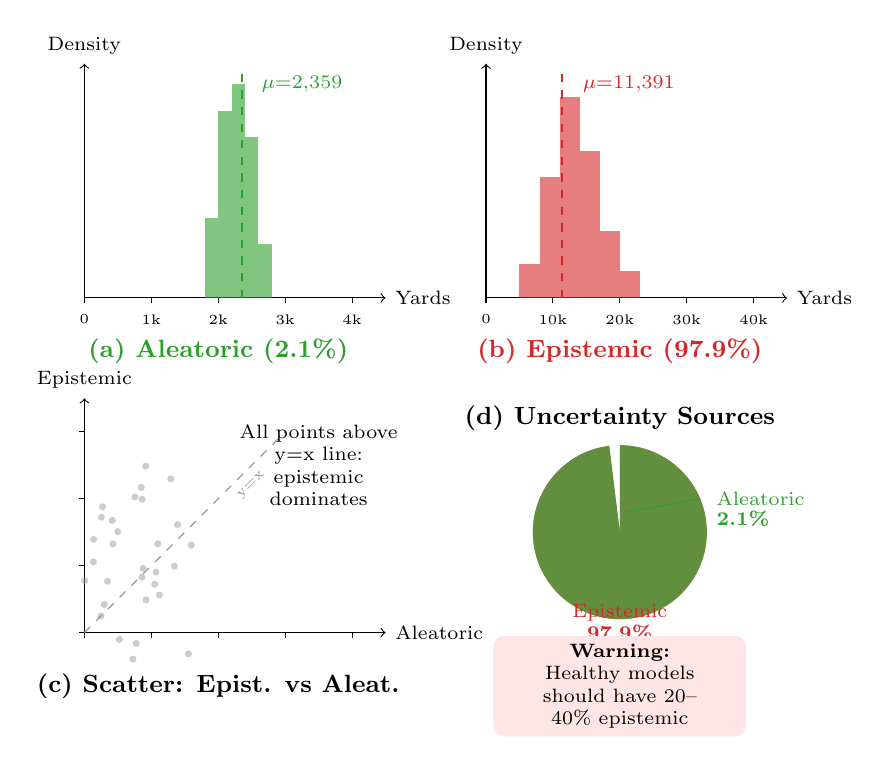
\begin{tikzpicture}[scale=0.85]
  % Define colors
  \definecolor{aleatoric}{RGB}{44,160,44}    % Green
  \definecolor{epistemic}{RGB}{214,39,40}    % Red
  \definecolor{total}{RGB}{148,103,189}      % Purple

  % ============================================
  % TOP LEFT: Aleatoric Uncertainty Distribution
  % ============================================
  \begin{scope}
    \draw[->] (0,0) -- (4.5,0) node[right, font=\scriptsize] {Yards};
    \draw[->] (0,0) -- (0,3.5) node[above, font=\scriptsize] {Density};

    % Histogram (narrow, centered at ~2,359)
    \fill[aleatoric, opacity=0.6] (1.8,0) rectangle (2.0, 1.2);
    \fill[aleatoric, opacity=0.6] (2.0,0) rectangle (2.2, 2.8);
    \fill[aleatoric, opacity=0.6] (2.2,0) rectangle (2.4, 3.2);
    \fill[aleatoric, opacity=0.6] (2.4,0) rectangle (2.6, 2.4);
    \fill[aleatoric, opacity=0.6] (2.6,0) rectangle (2.8, 0.8);

    % Mean line
    \draw[aleatoric, thick, dashed] (2.36, 0) -- (2.36, 3.4);
    \node[font=\scriptsize, aleatoric, anchor=west] at (2.5, 3.2) {$\mu$=2,359};

    % Axis ticks
    \foreach \x/\lab in {0/0, 1/1k, 2/2k, 3/3k, 4/4k} {
      \draw (\x, -0.08) -- (\x, 0);
      \node[below, font=\tiny] at (\x, -0.1) {\lab};
    }

    \node[font=\small\bfseries, aleatoric] at (2.0, -0.8) {(a) Aleatoric (2.1\%)};
  \end{scope}

  % ============================================
  % TOP RIGHT: Epistemic Uncertainty Distribution
  % ============================================
  \begin{scope}[xshift=6cm]
    \draw[->] (0,0) -- (4.5,0) node[right, font=\scriptsize] {Yards};
    \draw[->] (0,0) -- (0,3.5) node[above, font=\scriptsize] {Density};

    % Histogram (wide, centered at ~11,391)
    \fill[epistemic, opacity=0.6] (0.5,0) rectangle (0.8, 0.5);
    \fill[epistemic, opacity=0.6] (0.8,0) rectangle (1.1, 1.8);
    \fill[epistemic, opacity=0.6] (1.1,0) rectangle (1.4, 3.0);
    \fill[epistemic, opacity=0.6] (1.4,0) rectangle (1.7, 2.2);
    \fill[epistemic, opacity=0.6] (1.7,0) rectangle (2.0, 1.0);
    \fill[epistemic, opacity=0.6] (2.0,0) rectangle (2.3, 0.4);

    % Mean line
    \draw[epistemic, thick, dashed] (1.14, 0) -- (1.14, 3.4);
    \node[font=\scriptsize, epistemic, anchor=west] at (1.3, 3.2) {$\mu$=11,391};

    % Axis ticks (scale: 1 unit = 10k yards)
    \foreach \x/\lab in {0/0, 1/10k, 2/20k, 3/30k, 4/40k} {
      \draw (\x, -0.08) -- (\x, 0);
      \node[below, font=\tiny] at (\x, -0.1) {\lab};
    }

    \node[font=\small\bfseries, epistemic] at (2.0, -0.8) {(b) Epistemic (97.9\%)};
  \end{scope}

  % ============================================
  % BOTTOM LEFT: Epistemic vs Aleatoric Scatter
  % ============================================
  \begin{scope}[yshift=-5cm]
    \draw[->] (0,0) -- (4.5,0) node[right, font=\scriptsize] {Aleatoric};
    \draw[->] (0,0) -- (0,3.5) node[above, font=\scriptsize] {Epistemic};

    % Scatter points (epistemic >> aleatoric for all samples)
    \foreach \i in {1,...,30} {
      \pgfmathsetmacro{\ax}{0.8 + 0.8*rand}
      \pgfmathsetmacro{\ey}{1.0 + 1.5*rand}
      \fill[black!40, opacity=0.5] (\ax, \ey) circle (1.5pt);
    }

    % Reference line y=x
    \draw[dashed, black!40] (0,0) -- (3,3);
    \node[font=\tiny, rotate=45, black!40] at (2.5, 2.2) {y=x};

    % Annotation
    \node[font=\scriptsize, text width=2.5cm, align=center] at (3.5, 2.5) {All points above\\y=x line:\\epistemic\\dominates};

    % Axis ticks
    \foreach \x in {0,1,2,3,4} {
      \draw (\x, -0.08) -- (\x, 0);
    }
    \foreach \y in {0,1,2,3} {
      \draw (-0.08, \y) -- (0, \y);
    }

    \node[font=\small\bfseries] at (2.0, -0.8) {(c) Scatter: Epist. vs Aleat.};
  \end{scope}

  % ============================================
  % BOTTOM RIGHT: Pie Chart of Uncertainty Sources
  % ============================================
  \begin{scope}[xshift=6cm, yshift=-5cm]
    % Pie chart center
    \coordinate (center) at (2, 1.5);

    % Epistemic slice (97.9% = ~353 degrees)
    \fill[epistemic, opacity=0.7] (center) -- ++(90:1.3) arc (90:90-353:1.3) -- cycle;

    % Aleatoric slice (2.1% = ~7 degrees)
    \fill[aleatoric, opacity=0.7] (center) -- ++(90-353:1.3) arc (90-353:90:1.3) -- cycle;

    % Labels
    \node[font=\scriptsize, epistemic] at (2.0, 0.3) {Epistemic};
    \node[font=\scriptsize\bfseries, epistemic] at (2.0, 0.0) {97.9\%};

    \node[font=\scriptsize, aleatoric, anchor=west] at (3.3, 2.0) {Aleatoric};
    \node[font=\scriptsize\bfseries, aleatoric, anchor=west] at (3.3, 1.7) {2.1\%};
    \draw[aleatoric, thin] (2.1, 1.8) -- (3.2, 2.0);

    % Warning annotation
    \node[font=\scriptsize, text width=3cm, align=center, fill=red!10, rounded corners, inner sep=3pt] at (2.0, -0.8) {
      \textbf{Warning:} Healthy models\\should have 20--40\% epistemic
    };

    \node[font=\small\bfseries] at (2.0, 3.2) {(d) Uncertainty Sources};
  \end{scope}

\end{tikzpicture}
